\footnotetext{Exercises from Spivak (1965) Calculus on Manifolds}

\subsubsection*{2.2}
\begin{mdframed}
  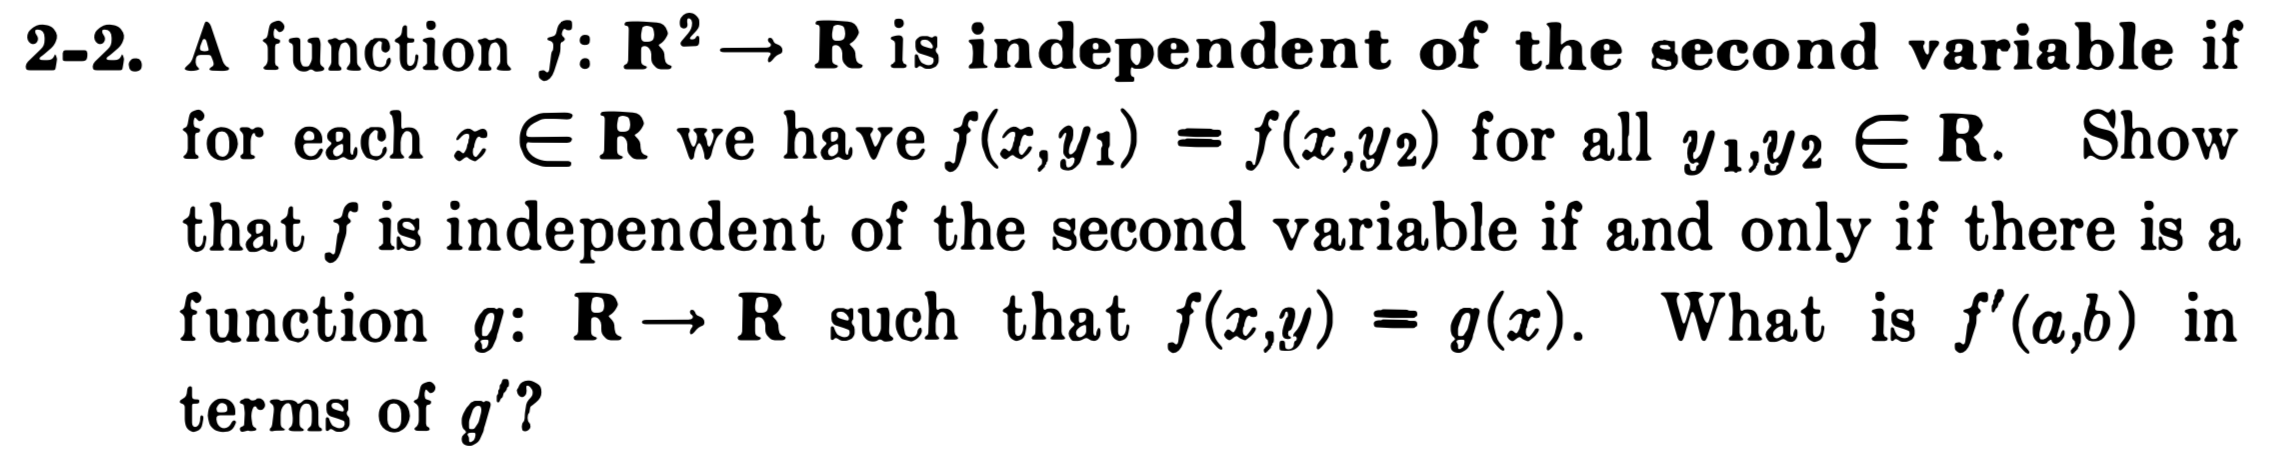
\includegraphics[width=400pt]{img/calculus-spivak--2-2.png}
\end{mdframed}
Suppose that $f$ is independent of its second argument. Fix $y \in \R$. Then there exists
$g:\R \to \R$ defined by $g(x) = f(x, y)$.

Conversely, suppose such a $g$ exists. If $f$ were not independent of its second argument then $g$
would not be a valid function.
\begin{align*}
  f'(a, b) &= ((D_1 f)(a, b), (D_2 f)(a, b)) \\
           &= (g'(a), 0).
\end{align*}
Check: We should have $f(a + h_1, b + h_2) \approx f(a, b) + f'(a, b) \cdot (h_1, h_2)^T$:
\begin{align*}
  f(a, b) + f'(a, b) \cdot (h_1, h_2)^T
  &= f(a, b) + (g'(a), 0) \cdot (h_1, h_2)^T \\
  &= f(a, b) + g'(a)\cdot h_1 + 0\cdot h_2
\end{align*}
